\documentclass[11pt,letterpaper]{article}
\usepackage[utf8]{inputenc}
\usepackage{caption} % for table captions
\usepackage{amsmath} % for multi-line equations and piecewises
\DeclareMathOperator{\sign}{sign}
\usepackage{graphicx}
\usepackage{relsize}
%\usepackage{textcomp}
\usepackage{xspace}
\usepackage{verbatim} % for block comments
%\usepackage{subfig} % for subfigures
\usepackage{enumitem} % for a) b) c) lists
\newcommand{\Cyclus}{\textsc{Cyclus}\xspace}%
\newcommand{\Cycamore}{\textsc{Cycamore}\xspace}%
\usepackage{tabularx}
\usepackage{color}
\usepackage[acronym,toc]{glossaries}
%\newacronym{<++>}{<++>}{<++>}
%\newacronym{<++>}{<++>}{<++>}
\newacronym[longplural={metric tons of heavy metal}]{MTHM}{MTHM}{metric ton of heavy metal}
\newacronym{ABM}{ABM}{agent-based modeling}
\newacronym{AHTR}{AHTR}{Advanced High Temperature Reactor}
\newacronym{ANDRA}{ANDRA}{Agence Nationale pour la gestion des D\'echets RAdioactifs, the French National Agency for Radioactive Waste Management}
\newacronym{ANL}{ANL}{Argonne National Laboratory}
\newacronym{API}{API}{application programming interface}
\newacronym{ARCH}{ARCH}{autoregressive conditional heteroskedastic}
\newacronym{ARE}{ARE}{Aircraft Reactor Experiment}
\newacronym{ARFC}{ARFC}{Advanced Reactors and Fuel Cycles}
\newacronym{ARMA}{ARMA}{autoregressive moving average}
\newacronym{ASME}{ASME}{American Society of Mechanical Engineers}
\newacronym{ATWS}{ATWS}{Anticipated Transient Without Scram}
\newacronym{BDBE}{BDBE}{Beyond Design Basis Event}
\newacronym{BIDS}{BIDS}{Berkeley Institute for Data Science}
\newacronym{CAFCA}{CAFCA}{ Code for Advanced Fuel Cycles Assessment }
\newacronym{CEA}{CEA}{Commissariat \`a l'\'Energie Atomique et aux \'Energies Alternatives}
\newacronym{CI}{CI}{continuous integration}
\newacronym{CNERG}{CNERG}{Computational Nuclear Engineering Research Group}
\newacronym{COSI}{COSI}{Commelini-Sicard}
\newacronym{COTS}{COTS}{commercial, off-the-shelf}
\newacronym{CSNF}{CSNF}{commercial spent nuclear fuel}
\newacronym{CTAH}{CTAHs}{Coiled Tube Air Heaters}
\newacronym{CUBIT}{CUBIT}{CUBIT Geometry and Mesh Generation Toolkit}
\newacronym{DAG}{DAG}{directed acyclic graph}
\newacronym{DANESS}{DANESS}{Dynamic Analysis of Nuclear Energy System Strategies}
\newacronym{DBE}{DBE}{Design Basis Event}
\newacronym{DESAE}{DESAE}{Dynamic Analysis of Nuclear Energy Systems Strategies}
\newacronym{DHS}{DHS}{Department of Homeland Security}
\newacronym{DOE}{DOE}{Department of Energy}
\newacronym{DRACS}{DRACS}{Direct Reactor Auxiliary Cooling System}
\newacronym{DRE}{DRE}{dynamic resource exchange}
\newacronym{DSNF}{DSNF}{DOE spent nuclear fuel}
\newacronym{DYMOND}{DYMOND}{Dynamic Model of Nuclear Development }
\newacronym{EBS}{EBS}{Engineered Barrier System}
\newacronym{EDZ}{EDZ}{Excavation Disturbed Zone}
\newacronym{EPA}{EPA}{Environmental Protection Agency}
\newacronym{EP}{EP}{Engineering Physics}
\newacronym{FCO}{FCO}{Fuel Cycle Options}
\newacronym{FCT}{FCT}{Fuel Cycle Technology}
\newacronym{FEHM}{FEHM}{Finite Element Heat and Mass Transfer}
\newacronym{FEPs}{FEPs}{Features, Events, and Processes}
\newacronym{FHR}{FHR}{Fluoride-Salt-Cooled High-Temperature Reactor}
\newacronym{FLiBe}{FLiBe}{Fluoride-Lithium-Beryllium}
\newacronym{GCAM}{GCAM}{Global Change Assessment Model}
\newacronym{GDSE}{GDSE}{Generic Disposal System Environment}
\newacronym{GDSM}{GDSM}{Generic Disposal System Model}
\newacronym{GENIUSv1}{GENIUSv1}{Global Evaluation of Nuclear Infrastructure Utilization Scenarios, Version 1}
\newacronym{GENIUSv2}{GENIUSv2}{Global Evaluation of Nuclear Infrastructure Utilization Scenarios, Version 2}
\newacronym{GENIUS}{GENIUS}{Global Evaluation of Nuclear Infrastructure Utilization Scenarios}
\newacronym{GPAM}{GPAM}{Generic Performance Assessment Model}
\newacronym{GRSAC}{GRSAC}{Graphite Reactor Severe Accident Code}
\newacronym{GUI}{GUI}{graphical user interface}
\newacronym{HLW}{HLW}{high level waste}
\newacronym{HPC}{HPC}{high-performance computing}
\newacronym{HTC}{HTC}{high-throughput computing}
\newacronym{HTGR}{HTGR}{High Temperature Gas-Cooled Reactor}
\newacronym{IAEA}{IAEA}{International Atomic Energy Agency}
\newacronym{INL}{INL}{Idaho National Laboratory}
\newacronym{JFNK}{JFNK}{Jacobian-Free Newton Krylov}
\newacronym{LANL}{LANL}{Los Alamos National Laboratory}
\newacronym{LBNL}{LBNL}{Lawrence Berkeley National Laboratory}
\newacronym{LCOE}{LCOE}{levelized cost of electricity}
\newacronym{LDRD}{LDRD}{laboratory directed research and development}
\newacronym{LFR}{LFR}{Lead-Cooled Fast Reactor}
\newacronym{LLNL}{LLNL}{Lawrence Livermore National Laboratory}
\newacronym{LMFBR}{LMFBR}{Liquid-Metal-cooled Fast Breeder Reactor}
\newacronym{LOFC}{LOFC}{Loss of Forced Cooling}
\newacronym{LOHS}{LOHS}{Loss of Heat Sink}
\newacronym{LOLA}{LOLA}{Loss of Large Area}
\newacronym{LP}{LP}{linear program}
\newacronym{MARKAL}{MARKAL}{MARKet and ALlocation}
\newacronym{MA}{MA}{minor actinide}
\newacronym{MCNP}{MCNP}{Monte Carlo N-Particle code}
\newacronym{MILP}{MILP}{mixed-integer linear program}
\newacronym{MIT}{MIT}{the Massachusetts Institute of Technology}
\newacronym{MOAB}{MOAB}{Mesh-Oriented datABase}
\newacronym{MOOSE}{MOOSE}{Multiphysics Object-Oriented Simulation Environment}
\newacronym{MOX}{MOX}{mixed oxide}
\newacronym{MSBR}{MSBR}{Molten Salt Breeder Reactor}
\newacronym{MSRE}{MSRE}{Molten Salt Reactor Experiment}
\newacronym{MSR}{MSR}{Molten Salt Reactor}
\newacronym{NAGRA}{NAGRA}{National Cooperative for the Disposal of Radioactive Waste}
\newacronym{NEAMS}{NEAMS}{Nuclear Engineering Advanced Modeling and Simulation}
\newacronym{NEUP}{NEUP}{Nuclear Energy University Programs}
\newacronym{NFCSim}{NFCSim}{Nuclear Fuel Cycle Simulator}
\newacronym{NFC}{NFC}{Nuclear Fuel Cycle}
\newacronym{NGNP}{NGNP}{Next Generation Nuclear Plant}
\newacronym{NNSA}{NNSA}{National Nuclear Security Administration}
\newacronym{NQA1}{NQA-1}{Nuclear Quality Assurance - 1}
\newacronym{NRC}{NRC}{Nuclear Regulatory Commission}
\newacronym{NSF}{NSF}{National Science Foundation}
\newacronym{NSSC}{NSSC}{Nuclear Science and Security Consortium}
\newacronym{NUWASTE}{NUWASTE}{Nuclear Waste Assessment System for Technical Evaluation}
\newacronym{NWTRB}{NWTRB}{Nuclear Waste Technical Review Board}
\newacronym{OCRWM}{OCRWM}{Office of Civilian Radioactive Waste Management}
\newacronym{ORION}{ORION}{ORION}
\newacronym{ORNL}{ORNL}{Oak Ridge National Laboratory}
\newacronym{PARCS}{PARCS}{Purdue Advanced Reactor Core Simulator}
\newacronym{PBAHTR}{PB-AHTR}{Pebble Bed Advanced High Temperature Reactor}
\newacronym{PBFHR}{PB-FHR}{Pebble-Bed Fluoride-Salt-Cooled High-Temperature Reactor}
\newacronym{PEI}{PEI}{Peak Environmental Impact}
\newacronym{PH}{PRONGHORN}{PRONGHORN}
\newacronym{PRKE}{PRKE}{Point Reactor Kinetics Equations}
\newacronym{PSPG}{PSPG}{Pressure-Stabilizing/Petrov-Galerkin}
\newacronym{PWAR}{PWAR}{Pratt and Whitney Aircraft Reactor}
\newacronym{PyNE}{PyNE}{Python toolkit for Nuclear Engineering}
\newacronym{PyRK}{PyRK}{Python for Reactor Kinetics}
\newacronym{QA}{QA}{quality assurance}
\newacronym{RDD}{RD\&D}{Research Development and Demonstration}
\newacronym{RD}{R\&D}{Research and Development}
\newacronym{RELAP}{RELAP}{Reactor Excursion and Leak Analysis Program}
\newacronym{RIA}{RIA}{Reactivity Insertion Accident}
\newacronym{RIF}{RIF}{Region-Institution-Facility}
\newacronym{SFR}{SFR}{Sodium-Cooled Fast Reactor}
\newacronym{SINDAG}{SINDA{\textbackslash}G}{Systems Improved Numerical Differencing Analyzer $\backslash$ Gaski}
\newacronym{SKB}{SKB}{Svensk K\"{a}rnbr\"{a}nslehantering AB}
\newacronym{SNF}{SNF}{spent nuclear fuel}
\newacronym{SNL}{SNL}{Sandia National Laboratory}
\newacronym{STC}{STC}{specific temperature change}
\newacronym{SUPG}{SUPG}{Streamline-Upwind/Petrov-Galerkin}
\newacronym{SWF}{SWF}{Separations and Waste Forms}
\newacronym{SWU}{SWU}{Separative Work Unit}
\newacronym{TRISO}{TRISO}{Tristructural Isotropic}
\newacronym{TSM}{TSM}{Total System Model}
\newacronym{TSPA}{TSPA}{Total System Performance Assessment for the Yucca Mountain License Application}
\newacronym{UFD}{UFD}{Used Fuel Disposition}
\newacronym{UML}{UML}{Unified Modeling Language}
\newacronym{UOX}{UOX}{uranium oxide}
\newacronym{UQ}{UQ}{uncertainty quantification}
\newacronym{US}{US}{United States}
\newacronym{UW}{UW}{University of Wisconsin}
\newacronym{VISION}{VISION}{the Verifiable Fuel Cycle Simulation Model}
\newacronym{VV}{V\&V}{verification and validation}
\newacronym{WIPP}{WIPP}{Waste Isolation Pilot Plant}
\newacronym{YMR}{YMR}{Yucca Mountain Repository Site}

\definecolor{bg}{rgb}{0.95,0.95,0.95}
\newcolumntype{b}{X}
\newcolumntype{f}{>{\hsize=.15\hsize}X}
\newcolumntype{s}{>{\hsize=.5\hsize}X}
\newcolumntype{m}{>{\hsize=.75\hsize}X}
\newcolumntype{r}{>{\hsize=1.1\hsize}X}
\usepackage{titling}
\usepackage[hang,flushmargin]{footmisc}
\renewcommand*\footnoterule{}
\usepackage[newfloat]{minted}
\newenvironment{code}{\captionsetup{type=listing}}{}
\SetupFloatingEnvironment{listing}{name=Code}
\newcolumntype{P}[1]{>{\centering\arraybackslash}p{#1}}

\bibliographystyle{abbrv}
\usepackage{tikz}


\usetikzlibrary{shapes.geometric,arrows}
\tikzstyle{process} = [rectangle, rounded corners, minimum width=1cm, minimum height=1cm,text centered, draw=black, fill=blue!30]
\tikzstyle{arrow} = [thick,->,>=stealth]


\graphicspath{{images/}}
\title{Numerical Experiments for Verifying Demand Driven Deployment Algorithms 
        \\ \vspace{0.5em} Non-Optimizing Algorithm}
\author{Jin Whan Bae, Gwendolyn J. Chee, Kathryn D. Huff}


\begin{document}
	\maketitle
	\hrule

\section{Project Objective}
The Demand-Driven Cycamore Archetype project (NEUP-FY16-10512) aims to develop \Cycamore's demand-driven deployment capabilities. The developed algorithm will be in the form of a \Cyclus \texttt{Institution} agent, and will deploy \texttt{Facilities} to meet the front-end and back-end demands of the fuel cycle.

\section{Motivation} 
The current \Cyclus fuel cycle simulation framework relies on the user to define
a deployment scheme or set the supporting \texttt{Facilities} capacities to infinity
to ensure that there's no gap in the nuclear fuel cycle supply chain. These user-defined assumptions 
are not an accurate reflection of the real world. 

\section{Method}
The project objective is met by developing three types of predictive algorithms: non-optimizing, deterministic-optimizing and stochastic-optimizing. Each algorithm aims to improve on the previous 
to provide more accurate prediction results.  

The prediction algorithms are being developed by the team at University of South Carolina. Meanwhile the numerical experiments are being designed by the team at University of Illinois at Urbana-Champaign.

This report will focus on the non-optimizing algorithm. 
It lists capability requirements of the non-optimizing case of the new \Cyclus \texttt{Institution}
for demand-driven deployment of fuel cycle facilities. 
It also discusses the tests to check correct implementation of the capabilities,
using a sample fuel cycle with well-defined facility parameters.

\section{Archetype Requirements}
Subsections \ref{subsection-user} to \ref{subsection-rate} state the requirements that apply to all three predictive algorithms. Expectations for the non-optimizing algorithm are different from expectations for the deterministic-optimizing and stochastic-optimizing algorithms. Therefore, in subsections \ref{subsection-deploy} to \ref{subsection-volatile}, the requirements unique to the non-optimizing algorithm are specified. 

\subsection{User Configuration}
\label{subsection-user}
The archetype should allow the user to define the following parameters: 
\begin{enumerate}
	\item A commodity whose demand drives deployment
	\item Initial amount of that commodity's demand
	\item Rate of growth or decline of that commodity's demand
	\item The facilities in the simulation able to meet that demand
	\item Algorithm type: non-optimizing, deterministic optimizing or stochastic optimizing
\end{enumerate}

\subsection{Create a supply chain}
\label{subsection-supplychain}
The archetype should be able to access the user defined parameters for the facilities in the simulation and evaluate if the commodities supplied by these facilities produce an appropriate supply chain to meet the demand of the commodity whose demand drives deployment. If not, the archetype should inform the user by throwing an error.  

\subsection{Growth Rate}
\label{subsection-rate}
The archetype should give the user options for different types of growth rate curves. Possible examples could be linear, exponential and piece-wise. 

\subsection{Facility Deployment and Decommissioning }
\label{subsection-deploy}
 The non-optimizing algorithm's deployment and decommissioning capabilities should be based on previous demand and supply values. At each time step, the algorithm should evaluate the demand for each commodity against its corresponding supply. If there is a shortage, the algorithm should deploy new facilities. If there is a surplus or more than one facility's capacity, the algorithm should decommission existing facilities. 
 
 \subsection{Dealing with volatility}
 \label{subsection-volatile}
A comprehensive fuel cycle simulator must have predictive capabilities which 
can deploy fuel cycle support facilities intelligently even in the face of 
volatile dynamics. If demand for the deployment-driving commodity is volatile, 
the archetype should recognize this. If it fails, the archetype would pathologically
deploy and decommission the same facility across short time periods due to volatile changes in commodity demand,
which is undesirable. 

\section{Simulation parameters for Test Scenarios}
Simple fuel cycle facilities populate the numerical testing of the algorithm.   

Table \ref{tab:testscenario} provides basic parameters for each test scenario. Table \ref{tab:reactor} provides the parameters for the \texttt{Source}, \texttt{Reactor} and \texttt{Sink} in the test scenarios.

\begin{table}[H]
	\centering
	\caption {Basic Test Parameters}
	\label{tab:testscenario}
	\begin{tabular}{|l|l|l|}
		\hline
		\textbf{Test Scenario Parameters} & \textbf{Value} & \textbf{Units} \\
		\hline
		Duration & 1000 & timesteps \\
		Timestep & 1 & month \\
		Start Month & 1 & month \\
		Start Year & 2000 & year \\
		\hline
	\end{tabular}
\end{table}

\begin{table}[H]
	\centering
    \caption {Source, Reactor and Sink Parameters}
	\label{tab:reactor}
	\begin{tabular}{|l|l|l|}
\hline
\textbf{Source Parameters} & \textbf{Value} & \textbf{Units} \\
\hline
Throughput & 1000 & kg \\
Output Commodity & fresh fuel & kg\\
\hline
\textbf{Reactor Parameters} & \textbf{Value} & \textbf{Units} \\
\hline
Cycle Time & 18 & timesteps \\
Refuel Time & 1 & timesteps \\
Lifetime & 500 & timesteps \\
Power Capacity & 1000 & MWe \\
Assembly Size & 1000 & kg \\
\# assemblies per core & 3 & \\
\# assemblies per batch & 1 & \\
Input Commodity & fresh fuel & kg\\
Output Commodities & power, spent fuel & MWe, kg\\
\hline
\textbf{Sink Parameters} & \textbf{Value} & \textbf{Units} \\
Throughput & 1000,000 & kg \\
Input Commodity & spent fuel & kg\\
\hline
	\end{tabular}
\end{table}

\pagebreak

\section{Numerical Tests for the Non-optimizing prediction method}
The tests are described based on the parameters defined in table \ref{tab:testscenario} and \ref{tab:reactor}. Every test is given facility and catch-up tolerances. Both tolerances are adjustable variables within the test script. Facility tolerance is the percentage difference that is considered acceptable for supply to differ from demand.  Catch-up tolerance is the number of time steps at the start of simulation that is considered acceptable for the supply of a commodity to not be within the acceptable range of it's demand. 

Therefore, each test is considered passed if the supply for every demanded commodity in the test scenario is within the facility tolerance of their demand at every time step, with exception to the initial catch-up tolerance.   

\subsection{Naming Convention for the numerical tests}

The naming convention of the numerical tests are in the form of \texttt{[Alphabet]}-\texttt{[Demand]}-\texttt{[Number]}. Each \texttt{Alphabet} refers to a scenario with a unique combination of \texttt{Facilities} and the commodity that drives deployment. Examples of scenarios that correspond to specific \texttt{Alphabets} is given in table \ref{tab:alphabet}. 
\begin{table}[H]
	\centering
	\caption {An \texttt{Alphabet} corresponding to each test scenario's \texttt{Facilities} and demand-driving commodity combination}
	\label{tab:alphabet}
	\begin{tabular}{|l|l|l|}
		\hline
		\texttt{Alphabet} & \textbf{Facilities in test scenario} & \textbf{\shortstack{Demand-driving \\ commodity}} \\
		\hline
		A & 1. Fresh fuel producing source facility & Fresh fuel \\
		\hline 
		B & \shortstack{1. Fresh fuel producing source facility \\ 2. Reactor facility } & Power \\
		\hline
		C & \shortstack{1. Fresh fuel producing source facility \\ 2. Reactor facility \\ 3. Sink facility } & Power \\
		\hline 
	\end{tabular}
\end{table}

The \texttt{Demand} component refers to the how the demand-driving commodity's demand changes over time. Examples of \texttt{Demand} types are \texttt{Constant}, \texttt{Growth} and \texttt{Decline}. The \texttt{Number} component refers to tests with the same \texttt{Alphabet} and \texttt{Demand}, but with other varying parameters.

\subsection{Numerical Tests}
\subsubsection{Test \texttt{[A]-[Constant]-[1]}}
The purpose of test \texttt{[A]-[Constant]-[1]} is to check if the non-optimizing algorithm works for the simplest scenario where there is only \texttt{Source} facilities available in the simulation to meet the constant demand of the demand-driving commodity: fresh fuel. 

Figure \ref{fig:test-a-constant-1-demand} shows the demand of the demand-driving commodity, fresh fuel, and the acceptable range for its supply during the entire simulation time.  

\begin{figure}[H]
	\begin{center}
		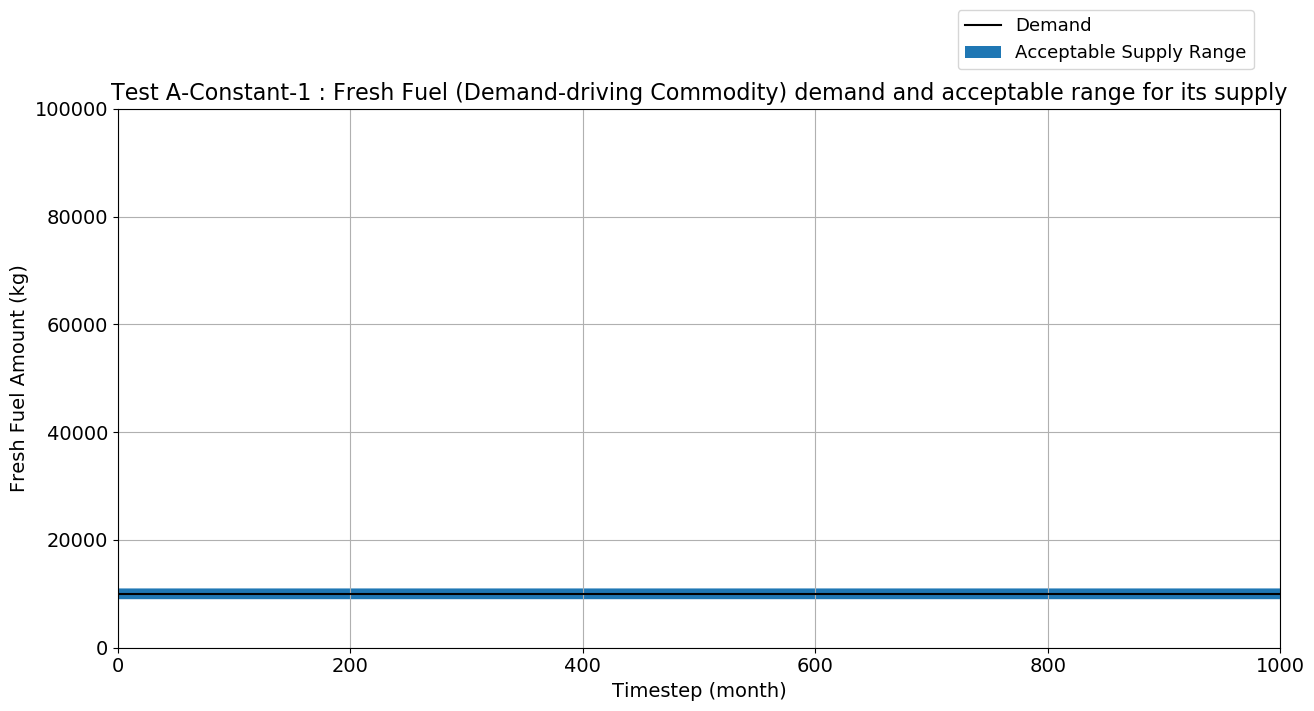
\includegraphics[scale=0.4]{./figures/demand_supply_A-Constant-1.png}
	\end{center}
        \caption{Fresh fuel demand for test A-const-1 and acceptable range for its supply.}
	\label{fig:test-a-constant-1-demand}
\end{figure}

\subsubsection{Test \texttt{[A]-[Growth]-[1]}}
The purpose of test \texttt{[A]-[Growth]-[1]} is to check if the non-optimizing algorithm works for a scenario where there are both \texttt{Source} and \texttt{Reactor} facilities available in the simulation to meet the linear growth of the demand-driving commodity: power. 

Figure \ref{fig:test-a-growth-1-demand} shows the demand of the demand-driving commodity, power, and the acceptable range for its supply during the entire simulation time.  

\begin{figure}[H]
	\begin{center}
		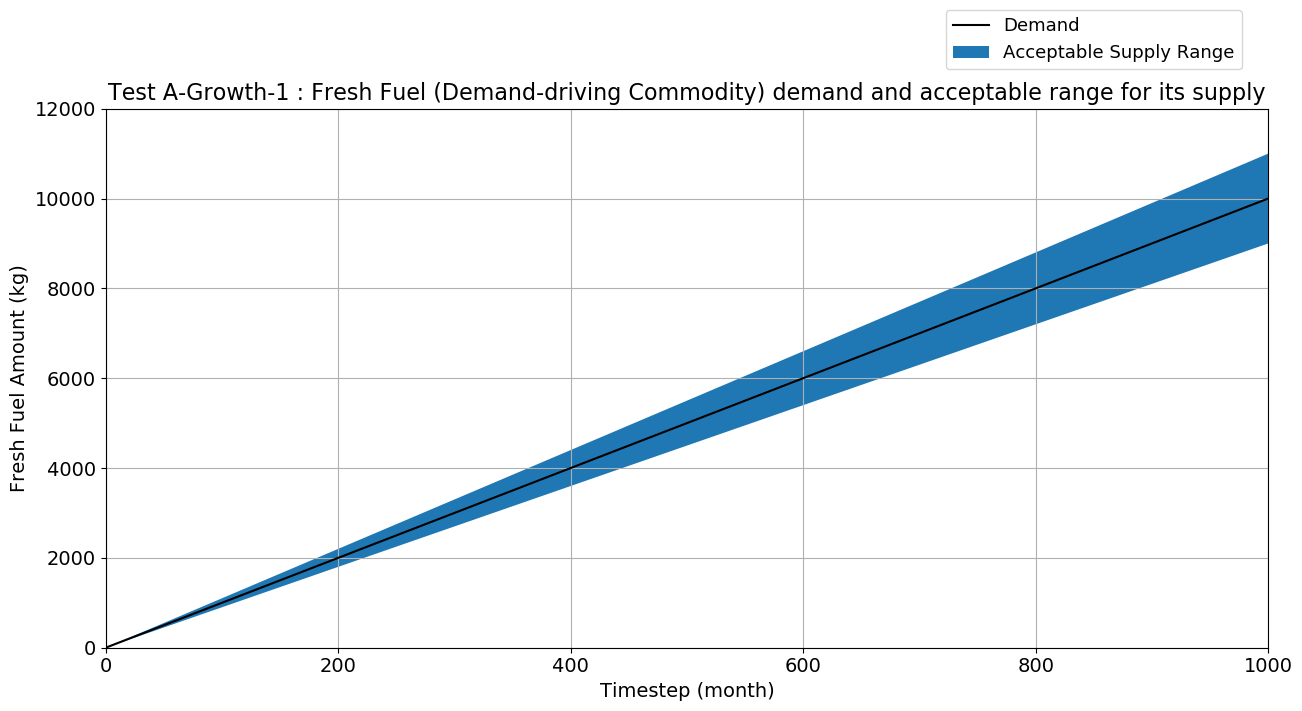
\includegraphics[scale=0.4]{./figures/demand_supply_A-Growth-1.png}
	\end{center}
        \caption{Power demand for test A-growth-1 and acceptable range for its supply.}
	\label{fig:test-a-growth-1-demand}
\end{figure}

\subsubsection{Test \texttt{[A]-[Growth]-[2]}}
The purpose of test \texttt{[A]-[Growth]-[2]} is to check if the non-optimizing algorithm works for a scenario where there are both \texttt{Source} and \texttt{Reactor} facilities available in the simulation to meet the exponential growth of the demand-driving commodity: power. 

Figure \ref{fig:test-a-growth-2-demand} shows the demand of the demand-driving commodity, power, and the acceptable range for its supply during the entire simulation time.  

\begin{figure}[H]
	\begin{center}
		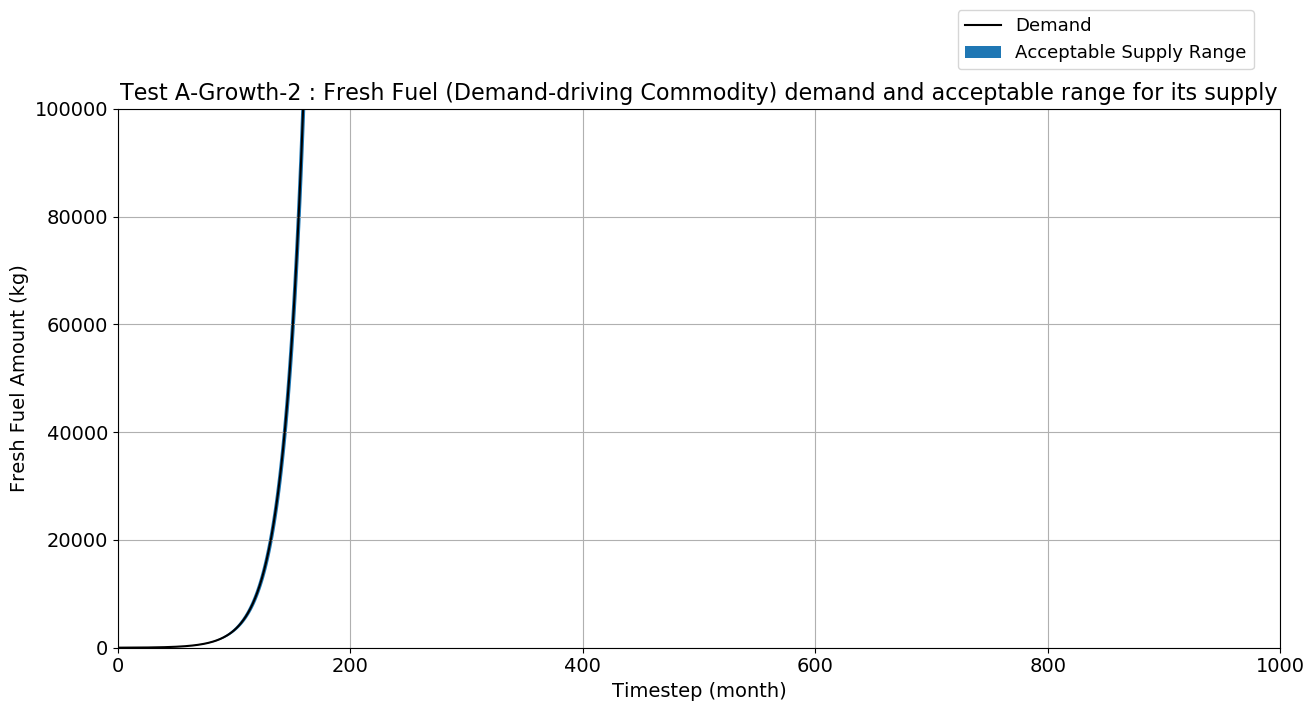
\includegraphics[scale=0.4]{./figures/demand_supply_A-Growth-2.png}
	\end{center}
        \caption{Power demand for test A-growth-2 and acceptable range for its supply.}
	\label{fig:test-a-growth-1-demand}
\end{figure}

\end{document}


